\documentclass[10pt]{article}
\usepackage[margin=1.7cm]{geometry}
\usepackage{graphicx}\usepackage{float}\usepackage{caption}
\graphicspath{{report_assets/}}
\title{\vspace{-1.5em}MLPC 2026 Task 5: Sound Event Detection Challenge}
\author{Quantized Transformers --- Aleksandr Masiev, Aleksandar Cvetkovic}
\date{}
\begin{document}\maketitle
\section*{Introduction}
We build a multi-label sound event detection (SED) system for MLPC 2026 Task 5 on the provided challenge dataset (3704 train, 999 validation, 1007 hidden-test recordings; 960 precomputed features per 1-second segment, 15 target classes). Following the baseline, an audio recording is cut into overlapping 1s segments (hop 0.5s); a multi-label classifier scores each segment and consecutive active whole-second segments are merged into onset/offset intervals. All numbers below are recomputed on the Task 5 dataset and scored with the official segment-based Macro F1 evaluator. We follow the baseline's seed-42 split of the provided validation set into a development-validation set (499 files, used for all tuning) and a non-hidden test set (500 files, used only for the final estimate). We do not attempt the bonus tasks (no raw waveforms were used).
\section*{1. Baseline Reproduction}
Method. We reproduce the provided baseline exactly: one DecisionTreeClassifier per class (max\_depth=20, max\_features='sqrt', random\_state=42) wrapped in a MultiOutputClassifier, trained on a 50,000-segment random subsample of raw (unscaled) features using the same rng sequence as the notebook. Result. On the non-hidden test set the baseline reaches Macro F1 = 0.316 (development validation 0.307). Class-wise it works best on loud, sustained sources (running\_water, vacuum\_cleaner, phone\_ringing, microwave) and worst on short or rare transients (window\_open\_close, wardrobe\_drawer\_open\_close, light\_switch). Strengths and limitations. The baseline is simple, fast and reproducible, and per-class binary trees handle polyphony naturally. However, (i) independent classifiers cannot model co-occurrence between classes; (ii) the 1-second resolution blurs short events and precise boundaries; (iii) hand-crafted segment statistics discard fine temporal structure; and (iv) a depth-limited tree on a 50k subsample under-fits a 960-dimensional, strongly imbalanced feature space, which caps recall on rare classes.
\begin{figure}[H]\centering
\includegraphics[width=0.95\linewidth]{fig_label_distribution.png}\caption*{\footnotesize Figure 8: Class imbalance in the training annotations.}\end{figure}
\section*{2. Simple Classifiers}
Previous best (Task 4). Our Task 4 best model was a one-vs-rest linear ridge classifier (alpha=2.0, decision threshold 0.50, balanced class weights, standardized features). We adapt this idea to the Task 5 SED pipeline: features are standardized on the training split only (no imputation -- the features contain zero NaNs), the ridge produces a per-segment score, a sigmoid maps it to [0,1], and a threshold yields per-second binary activity that is merged into intervals. Ridge is solved in closed form (weighted normal equations) for speed and numerical robustness. Hyperparameter study (36 configurations). We vary two important hyperparameters: the ridge regularisation alpha in \{0.1,0.5,1,2,5,10\} and the decision threshold in \{0,0.25,0.5,0.75\} (Fig. 3). We also evaluate one-vs-rest logistic regression (liblinear; regularisation C and class\_weight) and a RandomForest, tuning >=2 hyperparameters each. Best development-validation Macro F1 per family: ridge 0.410, logistic 0.432, random forest 0.391. Best classical model. logistic (C=1.0,class\_weight=None, threshold 0.3) gives non-hidden test Macro F1 = 0.436, versus the baseline's 0.316 -- an absolute gain of +0.120 (Fig. 1, Fig. 2). Largest per-class improvements: keyboard\_typing (0.36$\rightarrow$0.62), light\_switch (0.23$\rightarrow$0.43), microwave (0.39$\rightarrow$0.58), cutlery\_dishes (0.29$\rightarrow$0.46). Classes that remain hard: window\_open\_close (0.12), wardrobe\_drawer\_open\_close (0.16), door\_open\_close (0.31), bell\_ringing (0.32). The linear model benefits from standardisation, balanced weights and using all training segments, and the threshold trades precision against recall on imbalanced classes. Qualitative error analysis (Fig. 4-6, three non-hidden files). The success case detects the dominant sustained classes with good temporal overlap; the false-positive case shows extra short-transient activations (acoustically similar onsets) that hurt precision; the missed case shows short/rare events lost at 1-second resolution. Misses concentrate on rare classes and timing disagreements appear mostly at event boundaries, consistent with annotator label noise.
\begin{figure}[H]\centering
\includegraphics[width=0.6\linewidth]{fig_model_comparison.png}\caption*{\footnotesize Figure 1: Non-hidden test Macro F1 of the baseline, the best classical model, and after post-processing.}\end{figure}
\begin{figure}[H]\centering
\includegraphics[width=0.95\linewidth]{fig_per_class_f1.png}\caption*{\footnotesize Figure 2: Per-class F1 on the non-hidden test set.}\end{figure}
\begin{figure}[H]\centering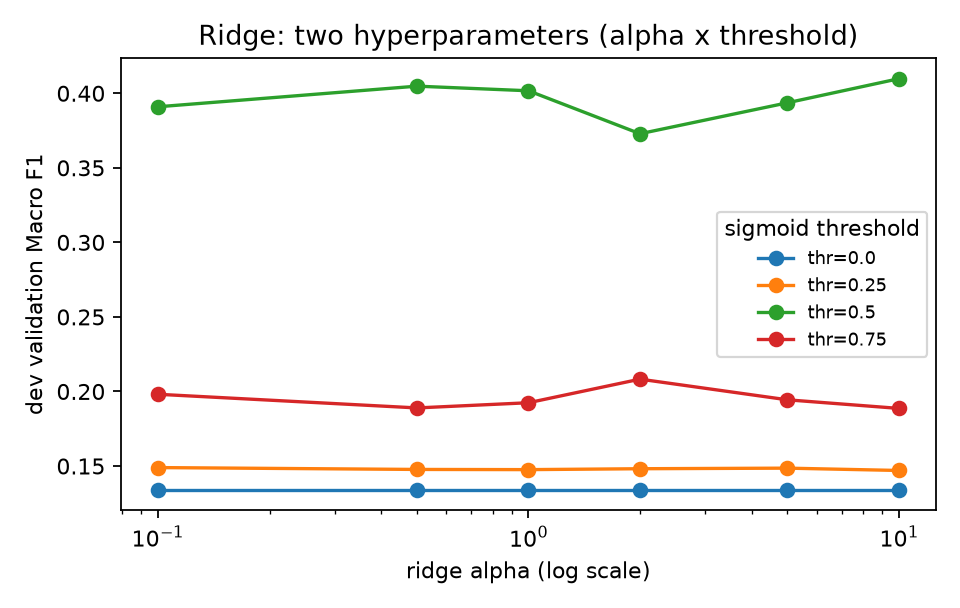
\includegraphics[width=0.6\linewidth]{fig_hyperparam.png}\caption*{\footnotesize Figure 3: Ridge hyperparameter study (alpha x sigmoid threshold) on development validation.}\end{figure}
\begin{figure}[H]\centering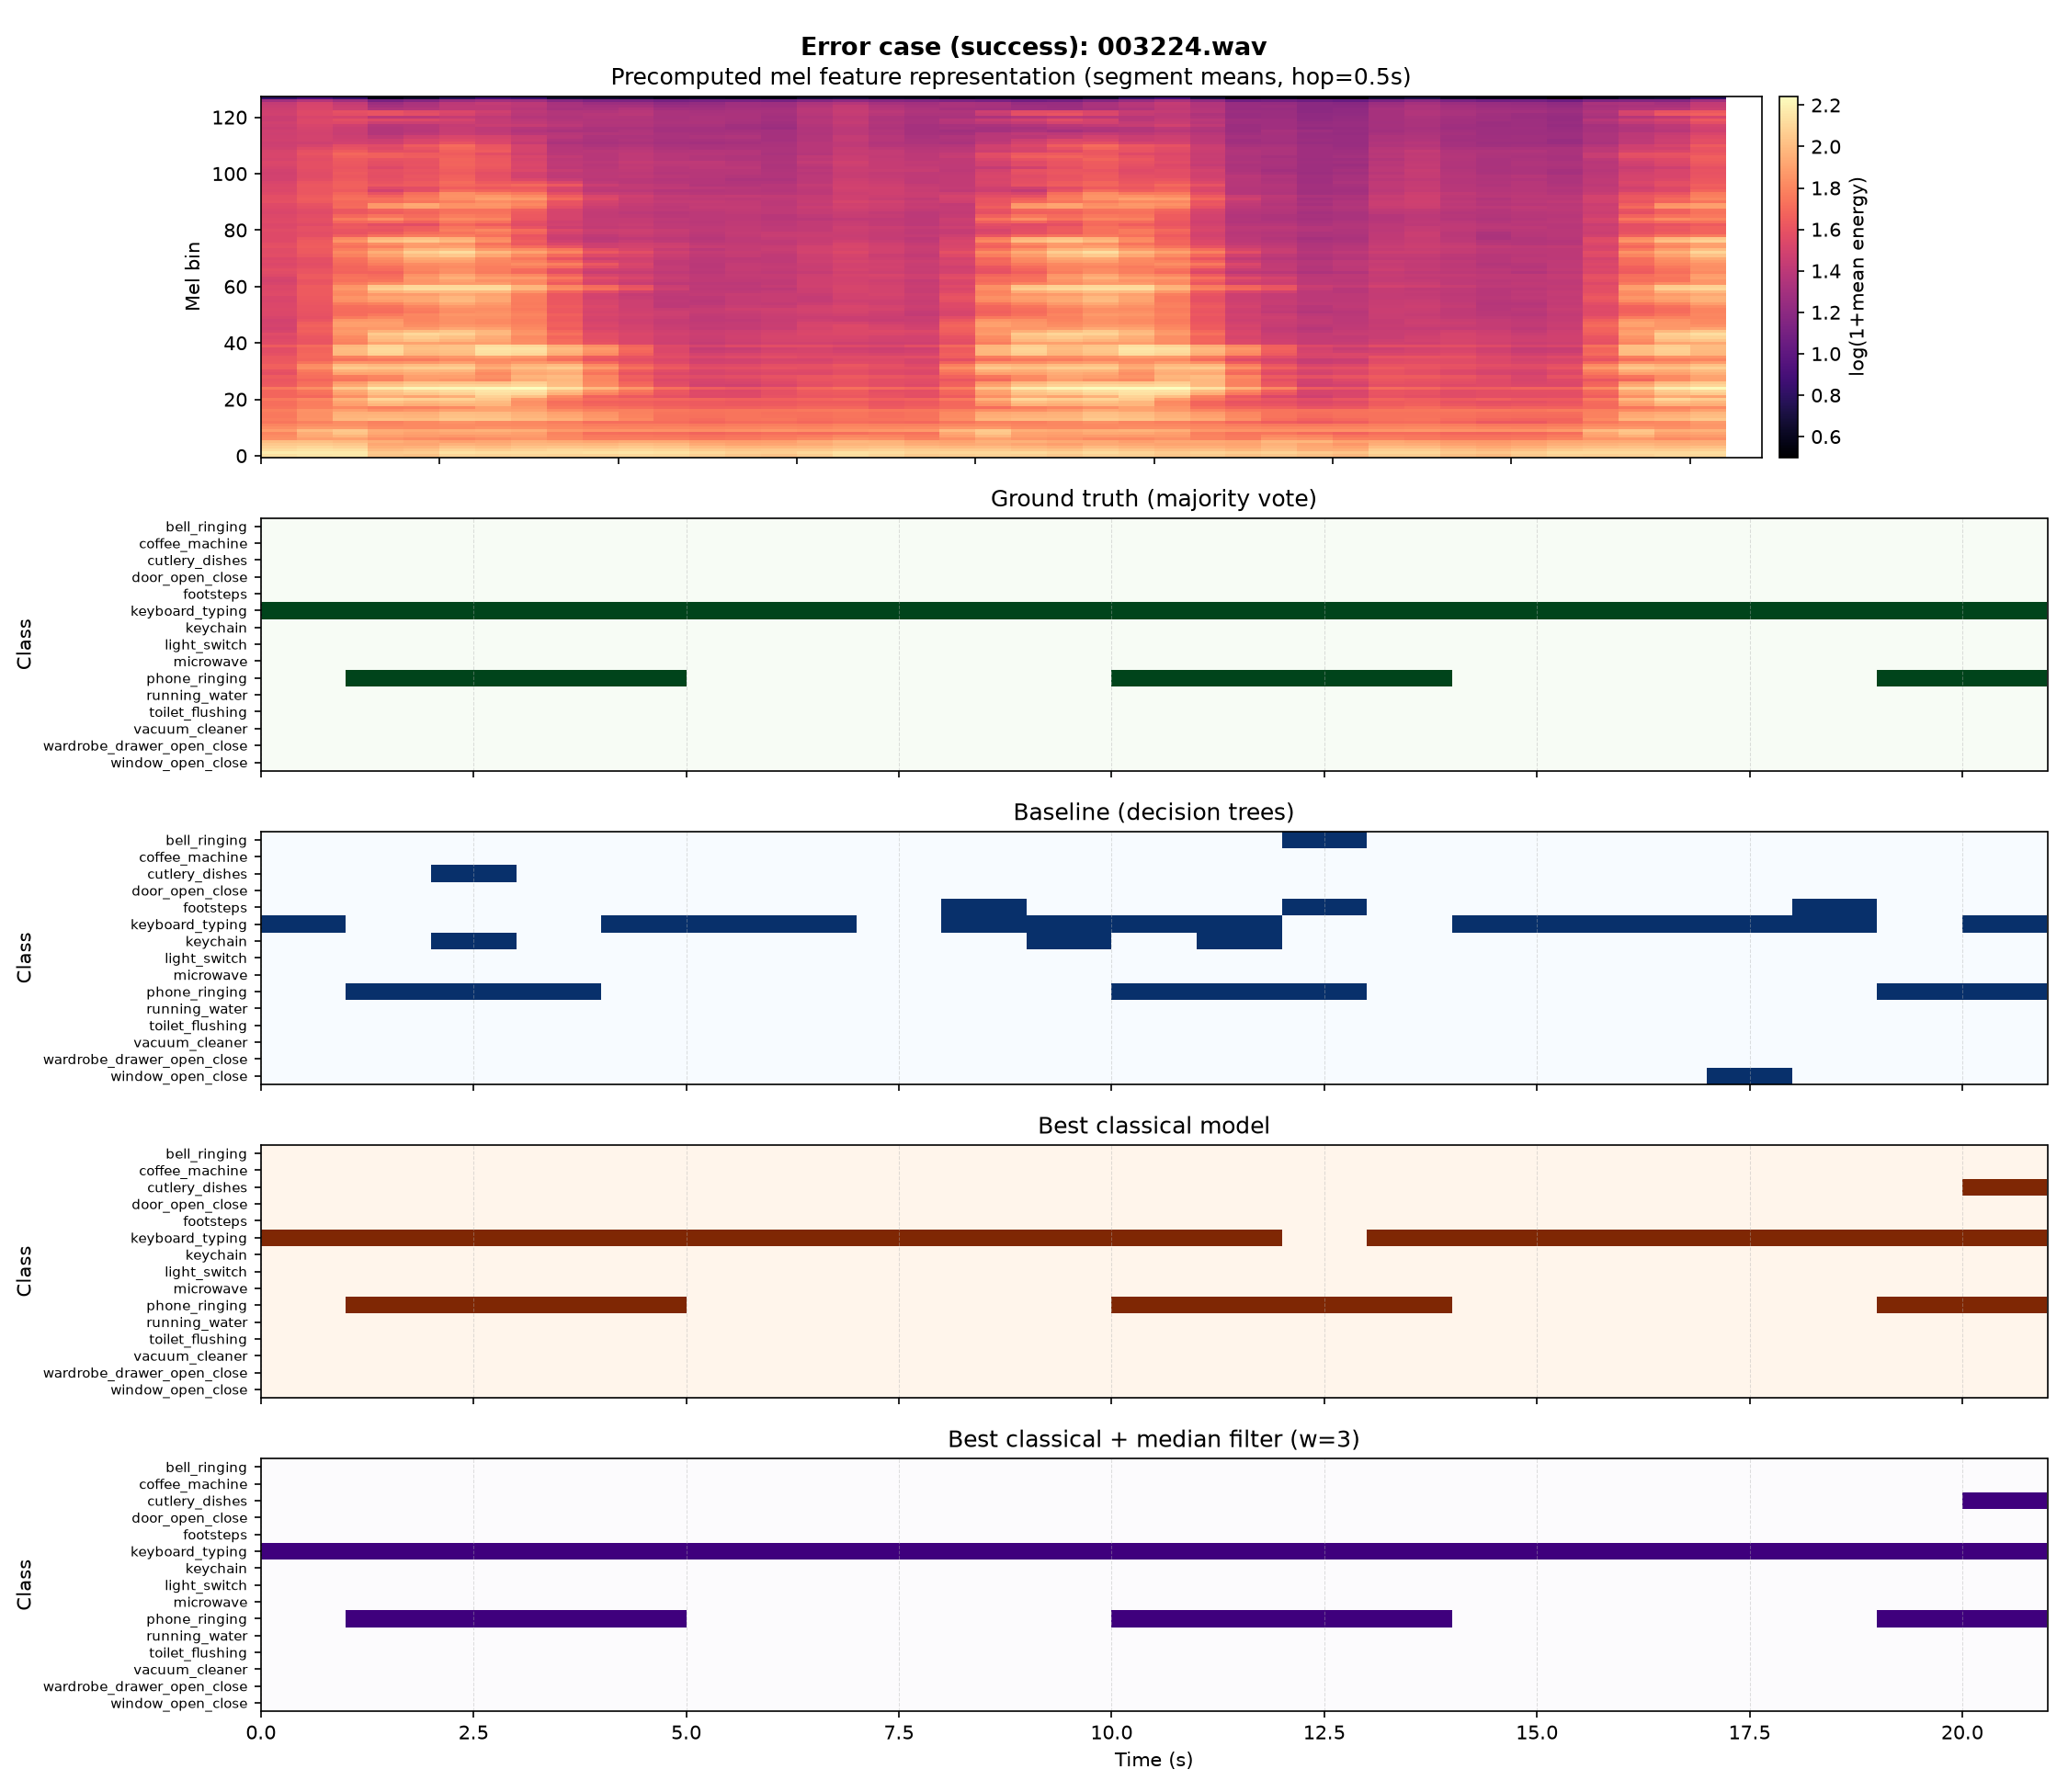
\includegraphics[width=0.95\linewidth]{error_case_1.png}\caption*{\footnotesize Figure 4: Error analysis -- success case (feature heatmap, GT, baseline, classical, post-processed).}\end{figure}
\begin{figure}[H]\centering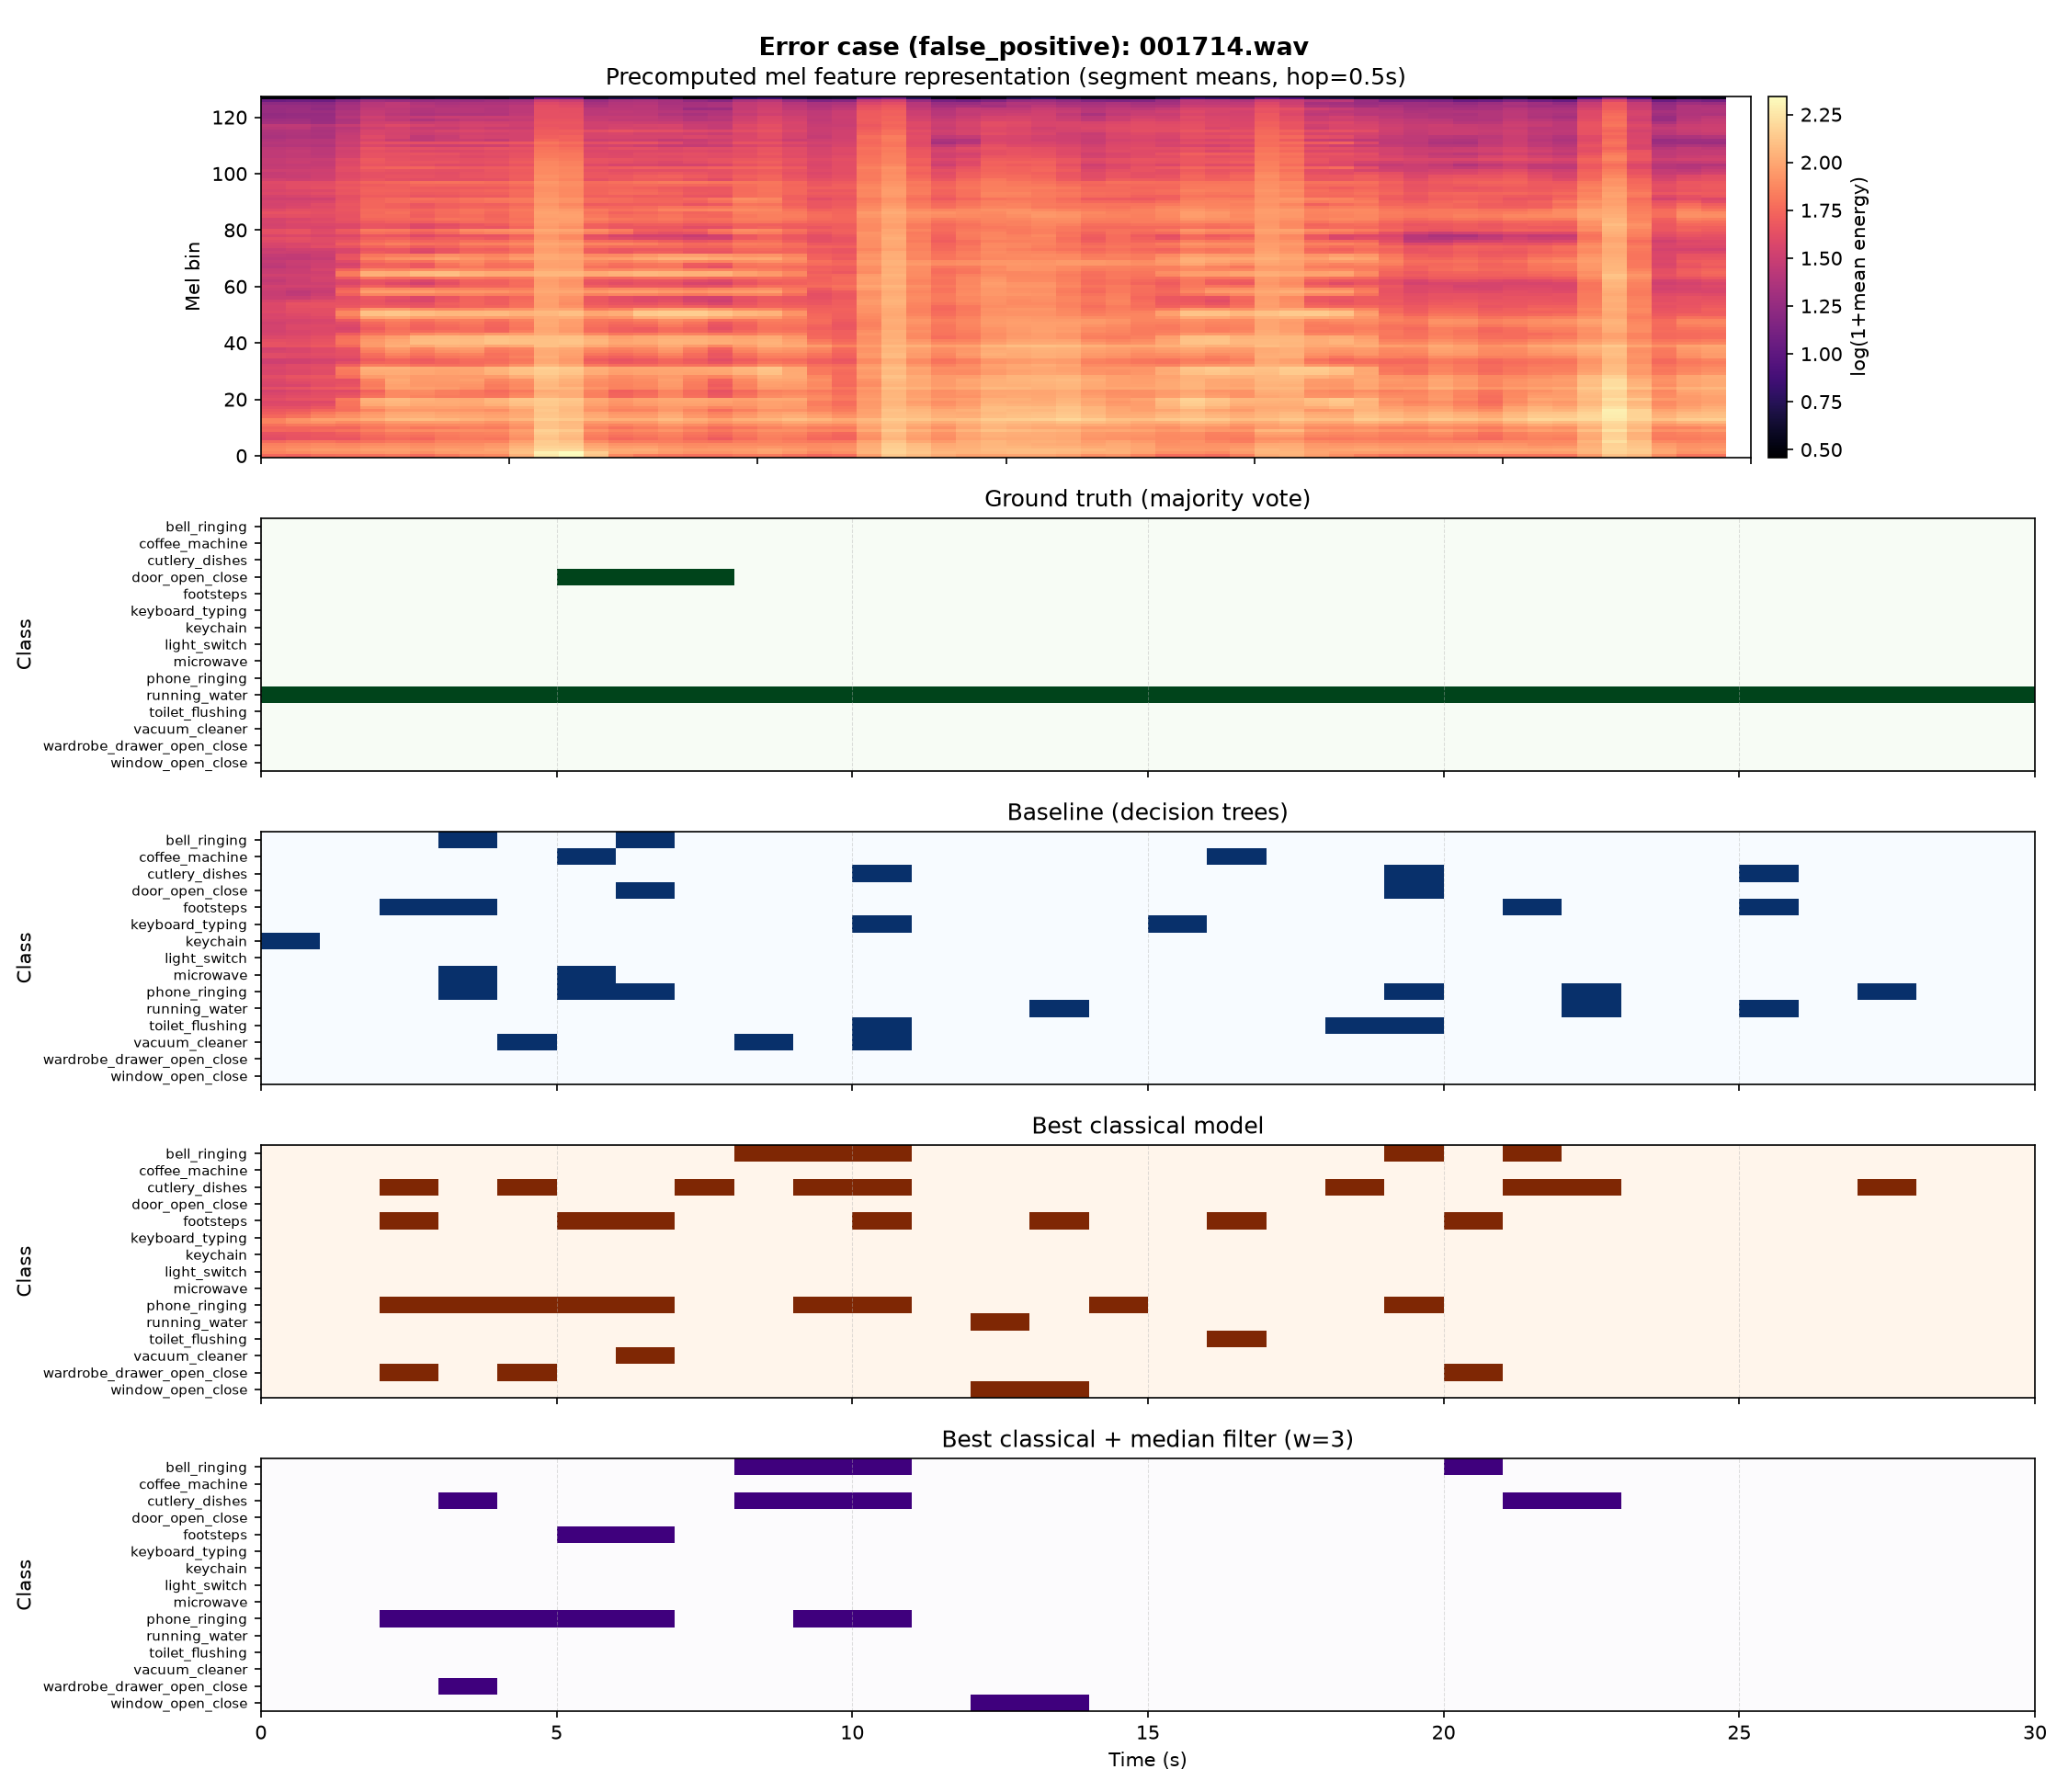
\includegraphics[width=0.95\linewidth]{error_case_2.png}\caption*{\footnotesize Figure 5: Error analysis -- false-positive / noisy case.}\end{figure}
\begin{figure}[H]\centering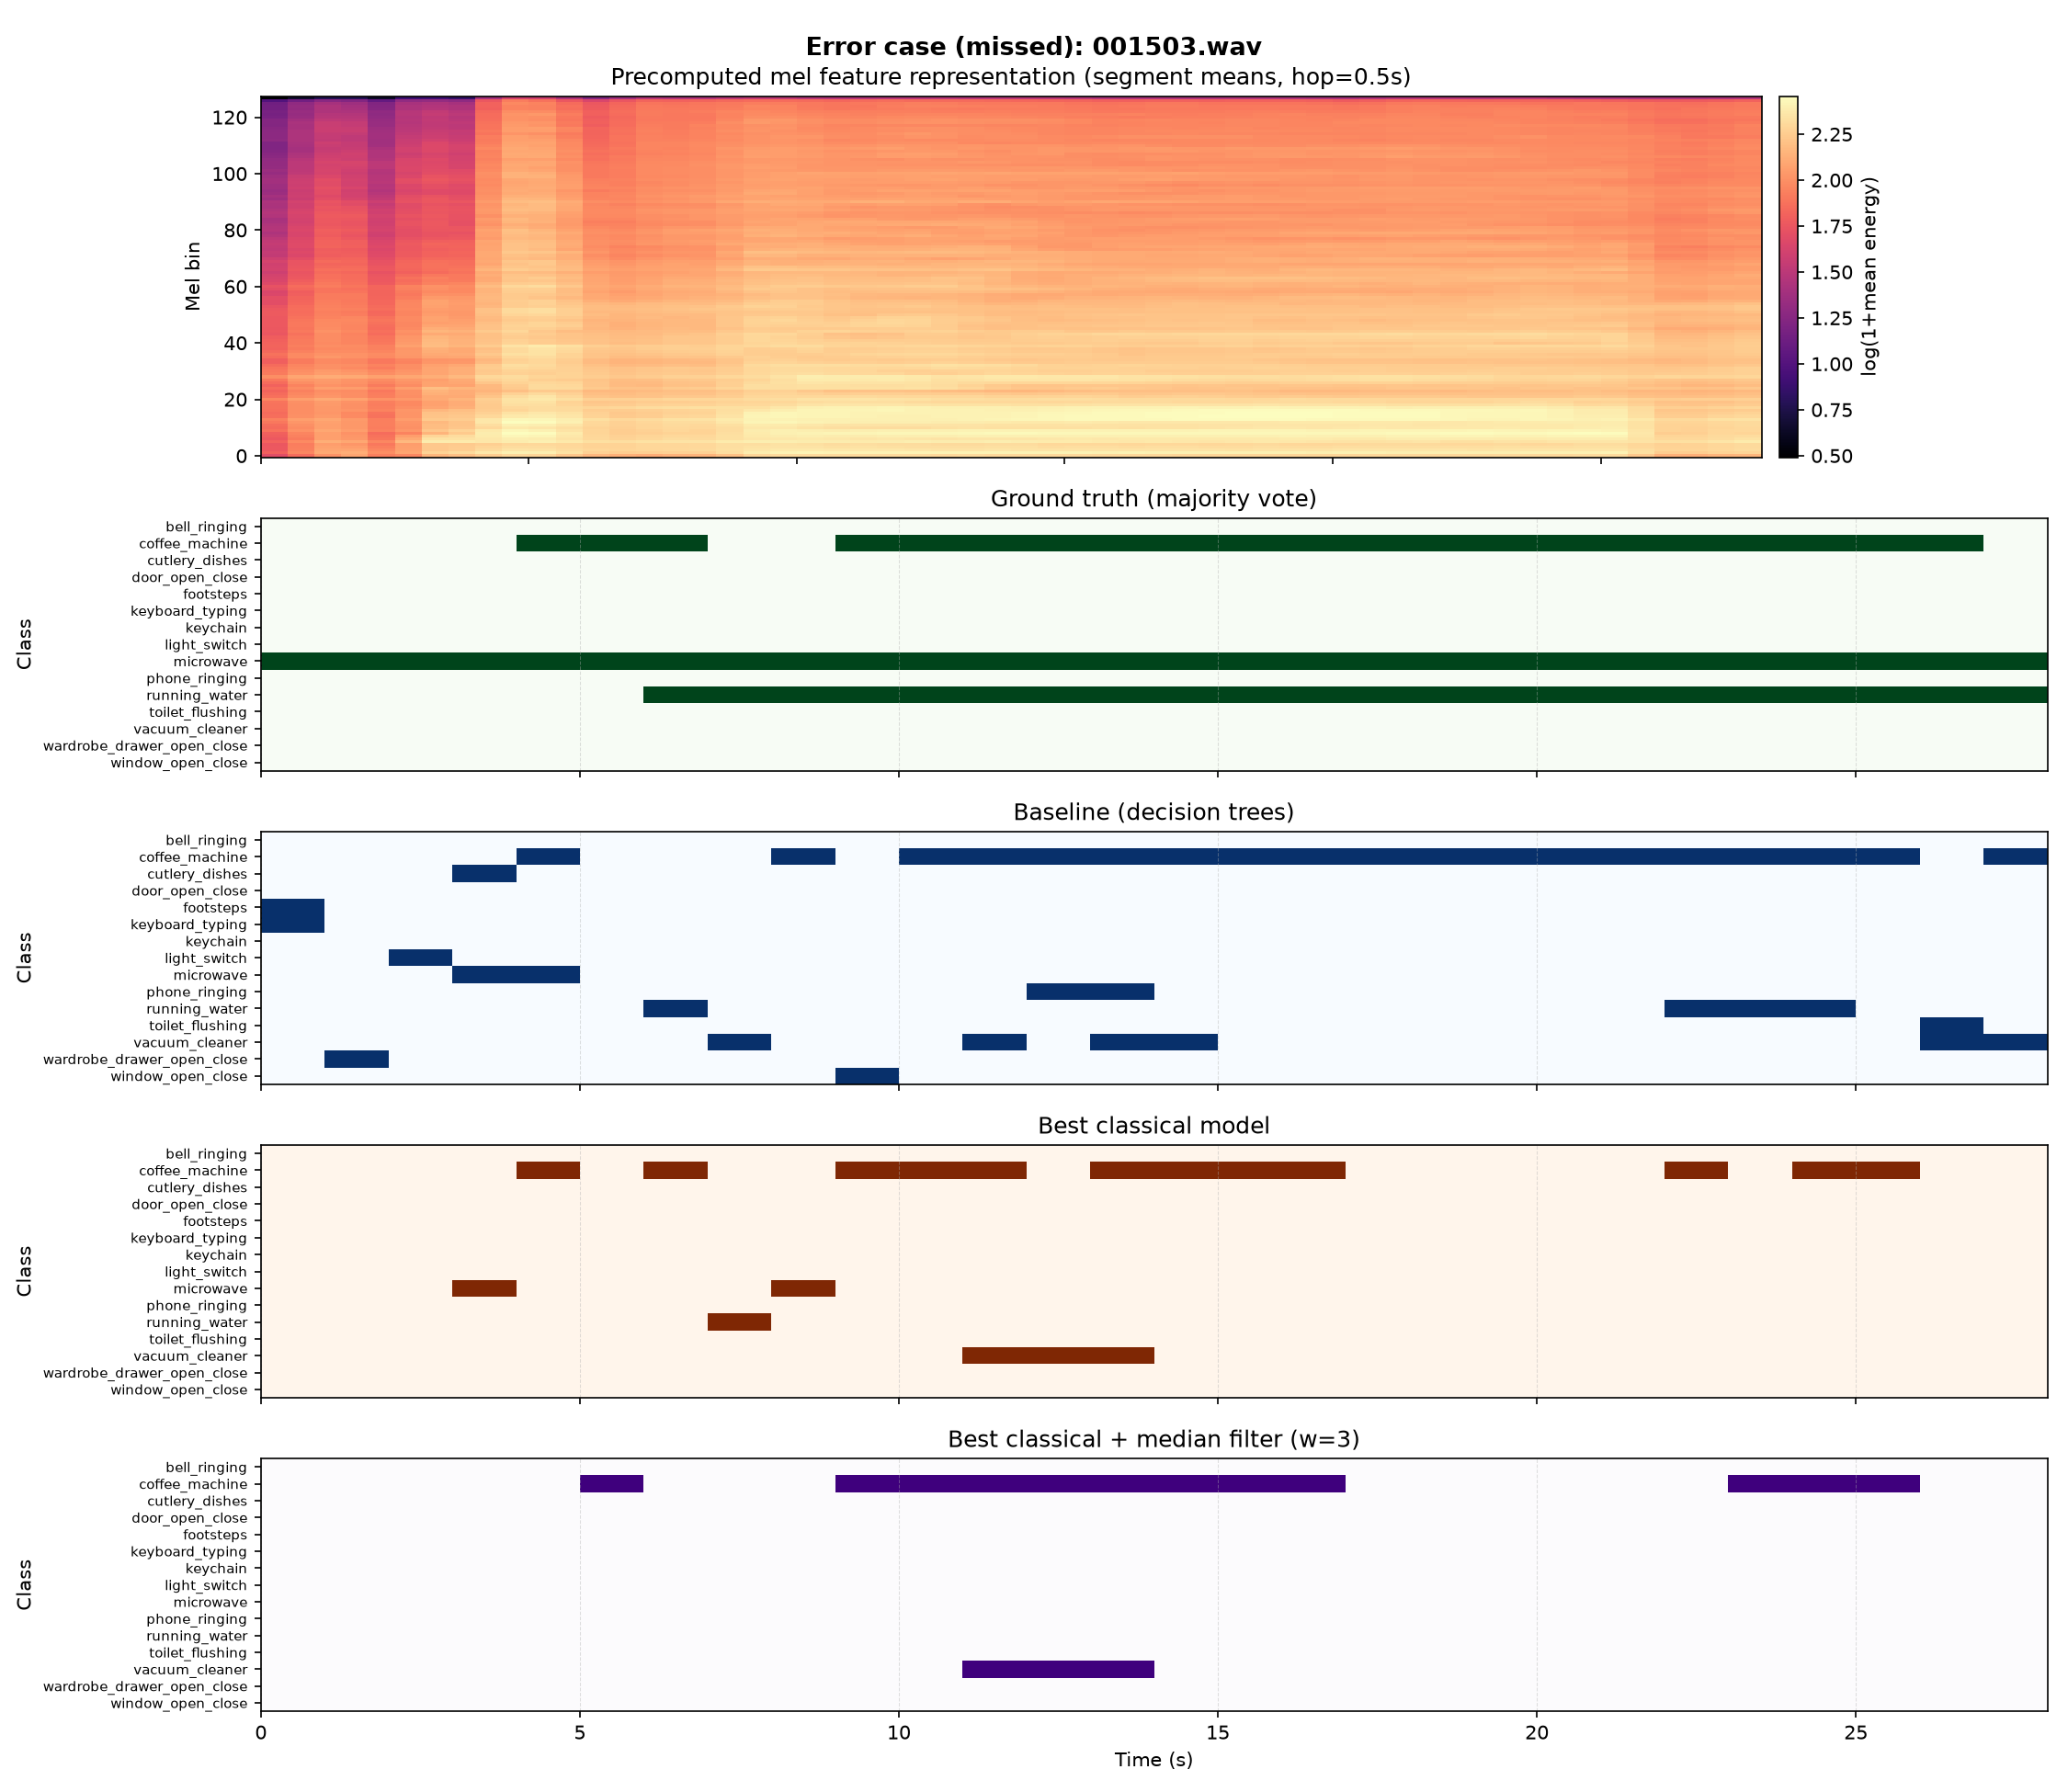
\includegraphics[width=0.95\linewidth]{error_case_3.png}\caption*{\footnotesize Figure 6: Error analysis -- missed-event / timing case.}\end{figure}
\section*{3. Post-Processing and Temporal Refinement}
Method. We apply a per-class temporal median filter to the per-second binary predictions before merging into intervals; it removes isolated false-positive blips and fills single-frame gaps. Window 1 means no post-processing. Parameter study. We select the window in \{1,3,5\} on the development validation set (Fig. 7) and evaluate the chosen window once on the non-hidden test set. Before/after. Selected window 3: non-hidden test Macro F1 goes from 0.436 (no post-processing) to 0.446. Median filtering reduced noisy false positives for sustained classes and slightly raised Macro F1; very short events can be smoothed away, so the gain is modest and class-dependent.
\begin{figure}[H]\centering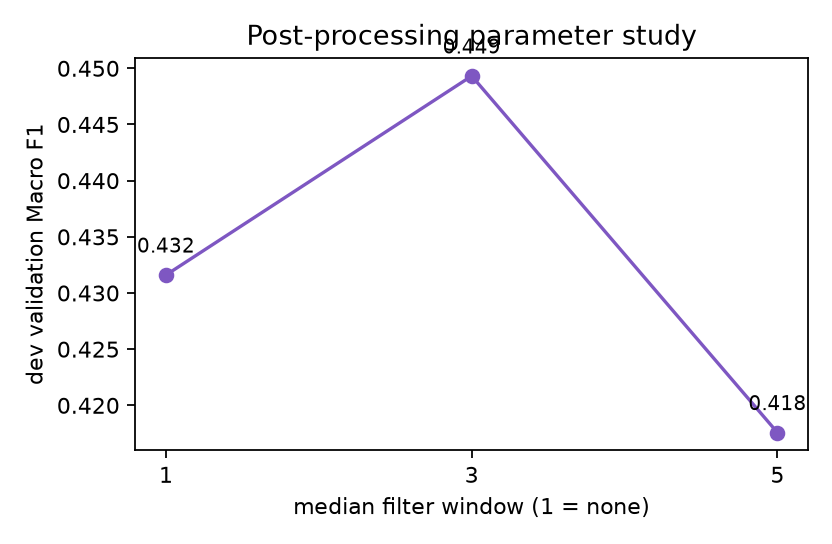
\includegraphics[width=0.6\linewidth]{fig_postproc.png}\caption*{\footnotesize Figure 7: Median-filter window selection on development validation.}\end{figure}
\section*{4. Reflection and Real-World Considerations}
Technical limitations. Independent linear per-class models ignore class co-occurrence and the 1-second segment statistics cannot localise short events precisely; performance is capped by label noise and strong class imbalance. Future improvements. Sequence models (e.g. a small temporal CNN/CRNN on the feature frames), per-class threshold calibration, feature selection, and richer temporal smoothing (e.g. hysteresis or HMM smoothing) are natural next steps. Smart-home deployment. A linear segment classifier is extremely cheap (a matrix multiply per second), giving low latency and low compute -- attractive for on-device inference. For reliability, precision matters: false alarms erode user trust, so per-class thresholds should be tuned to the use case, and robustness to unseen rooms, devices and background noise must be validated. Users expect consistent detection of salient events (doorbell, running water) more than perfect boundaries, which aligns with the segment-based metric.
\section*{5. Disclosure of LLM and AI Tool Use}
ChatGPT and Claude Code were used for brainstorming, coding assistance, debugging, and for structuring and improving the clarity of this report and the slides. All numerical results were produced by running our own code on the Task 5 challenge dataset and were verified with the official evaluation script (evaluate.py); no metrics were copied from Task 4. The final content was reviewed and understood by the students.
\end{document}